
% region CPBP bar graphs

% Bar graph representing the blue constraint's marginals on variable x
\newcommand{\blueGraphX}{
    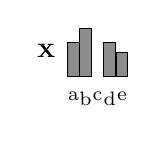
\begin{tikzpicture}
        \begin{axis}[
            ybar,
            axis y line=none,
            axis x line=bottom,
            axis line style={draw=none},
            ymin=0,
            ymax=100,
            width=2.2cm,
            height=2.2cm,
            bar width=1.5mm,
            xtick={a,b,c,d,e},
            xtick style={draw=none},
            symbolic x coords={a,b,c,d,e},
            xticklabel style={font=\scriptsize, anchor=north, yshift=-2pt},
            axis x line=bottom,
            axis y line=left,
            tick align=inside,
            enlarge x limits=0,
            clip=false,
        ]
            \addplot+[fill=gray!90, draw=black] coordinates {
                (a,70) (b,100) (d,70) (e,50)
            };
            \node[
                anchor=south east,
                font=\scriptsize\bfseries,
                xshift=-1mm, yshift=-5mm
            ] at (current axis.north west) {X};
        \end{axis}
    \end{tikzpicture}
}

% Bar graph representing the blue constraint's marginals on variable y
\newcommand{\blueGraphY}{
    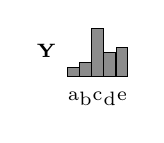
\begin{tikzpicture}
        \begin{axis}[
            ybar,
            axis y line=none,
            axis x line=bottom,
            axis line style={draw=none},
            ymin=0,
            ymax=100,
            width=2.2cm,
            height=2.2cm,
            bar width=1.5mm,
            xtick={a,b,c,d,e},
            xtick style={draw=none},
            symbolic x coords={a,b,c,d,e},
            xticklabel style={font=\scriptsize, anchor=north, yshift=-2pt},
            axis x line=bottom,
            axis y line=left,
            tick align=inside,
            enlarge x limits=0,
            clip=false,
        ]
            \addplot+[fill=gray!90, draw=black] coordinates {
                (a,20) (b,30) (c,100) (d,50) (e,60)
            };
            \node[
                anchor=south east,
                font=\scriptsize\bfseries,
                xshift=-1mm, yshift=-5mm
            ] at (current axis.north west) {Y};
        \end{axis}
    \end{tikzpicture}
}

% Bar graph representing the blue constraint's marginals on variable z
\newcommand{\blueGraphZ}{
    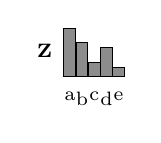
\begin{tikzpicture}
        \begin{axis}[
            ybar,
            axis y line=none,
            axis x line=bottom,
            axis line style={draw=none},
            ymin=0,
            ymax=100,
            width=2.2cm,
            height=2.2cm,
            bar width=1.5mm,
            xtick={a,b,c,d,e},
            xtick style={draw=none},
            symbolic x coords={a,b,c,d,e},
            xticklabel style={font=\scriptsize, anchor=north, yshift=-2pt},
            axis x line=bottom,
            axis y line=left,
            tick align=inside,
            enlarge x limits=0,
            clip=false,
        ]
            \addplot+[fill=gray!90, draw=black] coordinates {
                (a,100) (b,70) (c,30) (d,60) (e,20)
            };
            \node[
                anchor=south east,
                font=\scriptsize\bfseries,
                xshift=-1mm, yshift=-5mm
            ] at (current axis.north west) {Z};
        \end{axis}
    \end{tikzpicture}
}

% Bar graph representing the red constraint's marginals on variable x
\newcommand{\redGraphX}{
    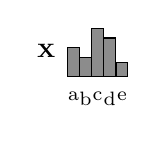
\begin{tikzpicture}
        \begin{axis}[
            ybar,
            axis y line=none,
            axis x line=bottom,
            axis line style={draw=none},
            ymin=0,
            ymax=100,
            width=2.2cm,
            height=2.2cm,
            bar width=1.5mm,
            xtick={a,b,c,d,e},
            xtick style={draw=none},
            symbolic x coords={a,b,c,d,e},
            xticklabel style={font=\scriptsize, anchor=north, yshift=-2pt},
            axis x line=bottom,
            axis y line=left,
            tick align=inside,
            enlarge x limits=0,
            clip=false,
        ]
            \addplot+[fill=gray!90, draw=black] coordinates {
                (a,60) (b,40) (c,100) (d,80) (e,30)
            };
            \node[
                anchor=south east,
                font=\scriptsize\bfseries,
                xshift=-1mm, yshift=-5mm
            ] at (current axis.north west) {X};
        \end{axis}
    \end{tikzpicture}
}

% Bar graph representing the red constraint's marginals on variable w
\newcommand{\redGraphW}{
    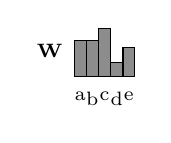
\begin{tikzpicture}
        \begin{axis}[
            ybar,
            axis y line=none,
            axis x line=bottom,
            axis line style={draw=none},
            ymin=0,
            ymax=100,
            width=2.2cm,
            height=2.2cm,
            bar width=1.5mm,
            xtick={a,b,c,d,e},
            xtick style={draw=none},
            symbolic x coords={a,b,c,d,e},
            xticklabel style={font=\scriptsize, anchor=north, yshift=-2pt},
            axis x line=bottom,
            axis y line=left,
            tick align=inside,
            enlarge x limits=0,
            clip=false,
        ]
            \addplot+[fill=gray!90, draw=black] coordinates {
                (a,75) (b,75) (c,100) (d,30) (e,60)
            };
            \node[
                anchor=south east,
                font=\scriptsize\bfseries,
                xshift=-1mm, yshift=-5mm
            ] at (current axis.north west) {W};
        \end{axis}
    \end{tikzpicture}
}

% Bar graph representing the red constraint's marginals on variable z
\newcommand{\redGraphZ}{
    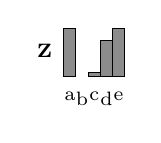
\begin{tikzpicture}
        \begin{axis}[
            ybar,
            axis y line=none,
            axis x line=bottom,
            axis line style={draw=none},
            ymin=0,
            ymax=100,
            width=2.2cm,
            height=2.2cm,
            bar width=1.5mm,
            xtick={a,b,c,d,e},
            xtick style={draw=none},
            symbolic x coords={a,b,c,d,e},
            xticklabel style={font=\scriptsize, anchor=north, yshift=-2pt},
            axis x line=bottom,
            axis y line=left,
            tick align=inside,
            enlarge x limits=0,
            clip=false,
        ]
            \addplot+[fill=gray!90, draw=black] coordinates {
                (a,100) (c,10) (d,75) (e,100)
            };
            \node[
                anchor=south east,
                font=\scriptsize\bfseries,
                xshift=-1mm, yshift=-5mm
            ] at (current axis.north west) {Z};
        \end{axis}
    \end{tikzpicture}
}

% endregion

% region Standard CP bar graphs

\newcommand{\blueCPX}{
    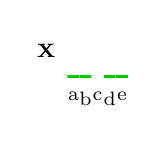
\begin{tikzpicture}
        \begin{axis}[
            ybar,
            axis y line=none,
            axis x line=bottom,
            axis line style={draw=none},
            ymin=0,
            ymax=100,
            width=2.2cm,
            height=2.2cm,
            bar width=1.5mm,
            xtick={a,b,c,d,e},
            xtick style={draw=none},
            symbolic x coords={a,b,c,d,e},
            xticklabel style={font=\scriptsize, anchor=north, yshift=-2pt},
            tick align=inside,
            enlarge x limits=0,
            clip=false,
        ]
            \addplot+[draw=none, fill=none, forget plot] coordinates {(e,100)};
            \addplot+[draw=green!80!black, very thick] coordinates {
            (a,0) (b,0) (d,0) (e,0)
            };

            % Label
            \node[
            anchor=south east,
            font=\scriptsize\bfseries,
            xshift=-1mm, yshift=-5mm
            ] at (current axis.north west) {X};

        \end{axis}
    \end{tikzpicture}
}

\newcommand{\blueCPY}{
    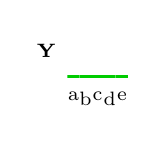
\begin{tikzpicture}
        \begin{axis}[
            ybar,
            axis y line=none,
            axis x line=bottom,
            axis line style={draw=none},
            ymin=0,
            ymax=100,
            width=2.2cm,
            height=2.2cm,
            bar width=1.5mm,
            xtick={a,b,c,d,e},
            xtick style={draw=none},
            symbolic x coords={a,b,c,d,e},
            xticklabel style={font=\scriptsize, anchor=north, yshift=-2pt},
            tick align=inside,
            enlarge x limits=0,
            clip=false,
        ]
            \addplot+[draw=none, fill=none, forget plot] coordinates {(e,100)};
            \addplot+[draw=green!80!black, very thick] coordinates {
            (a,0) (b,0) (c,0) (d,0) (e,0)
            };

            % Label
            \node[
            anchor=south east,
            font=\scriptsize\bfseries,
            xshift=-1mm, yshift=-5mm
            ] at (current axis.north west) {Y};

        \end{axis}
    \end{tikzpicture}
}

\newcommand{\blueCPZ}{
    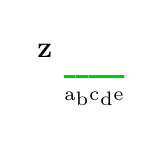
\begin{tikzpicture}
        \begin{axis}[
            ybar,
            axis y line=none,
            axis x line=bottom,
            axis line style={draw=none},
            ymin=0,
            ymax=100,
            width=2.2cm,
            height=2.2cm,
            bar width=1.5mm,
            xtick={a,b,c,d,e},
            xtick style={draw=none},
            symbolic x coords={a,b,c,d,e},
            xticklabel style={font=\scriptsize, anchor=north, yshift=-2pt},
            tick align=inside,
            enlarge x limits=0,
            clip=false,
        ]
            \addplot+[draw=none, fill=none, forget plot] coordinates {(e,100)};
            \addplot+[draw=green!80!black, very thick] coordinates {
            (a,0) (b,0) (c,0) (d,0) (e,0)
            };

            % Label
            \node[
            anchor=south east,
            font=\scriptsize\bfseries,
            xshift=-1mm, yshift=-5mm
            ] at (current axis.north west) {Z};

        \end{axis}
    \end{tikzpicture}
}

\newcommand{\redCPX}{
    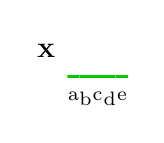
\begin{tikzpicture}
        \begin{axis}[
            ybar,
            axis y line=none,
            axis x line=bottom,
            axis line style={draw=none},
            ymin=0,
            ymax=100,
            width=2.2cm,
            height=2.2cm,
            bar width=1.5mm,
            xtick={a,b,c,d,e},
            xtick style={draw=none},
            symbolic x coords={a,b,c,d,e},
            xticklabel style={font=\scriptsize, anchor=north, yshift=-2pt},
            tick align=inside,
            enlarge x limits=0,
            clip=false,
        ]
            \addplot+[draw=none, fill=none, forget plot] coordinates {(e,100)};
            \addplot+[draw=green!80!black, very thick] coordinates {
            (a,0) (b,0) (c,0) (d,0) (e,0)
            };

            % Label
            \node[
            anchor=south east,
            font=\scriptsize\bfseries,
            xshift=-1mm, yshift=-5mm
            ] at (current axis.north west) {X};

        \end{axis}
    \end{tikzpicture}
}

\newcommand{\redCPW}{
    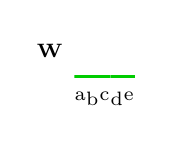
\begin{tikzpicture}
        \begin{axis}[
            ybar,
            axis y line=none,
            axis x line=bottom,
            axis line style={draw=none},
            ymin=0,
            ymax=100,
            width=2.2cm,
            height=2.2cm,
            bar width=1.5mm,
            xtick={a,b,c,d,e},
            xtick style={draw=none},
            symbolic x coords={a,b,c,d,e},
            xticklabel style={font=\scriptsize, anchor=north, yshift=-2pt},
            tick align=inside,
            enlarge x limits=0,
            clip=false,
        ]
            \addplot+[draw=none, fill=none, forget plot] coordinates {(e,100)};
            \addplot+[draw=green!80!black, very thick] coordinates {
            (a,0) (b,0) (c,0) (d,0) (e,0)
            };

            % Label
            \node[
            anchor=south east,
            font=\scriptsize\bfseries,
            xshift=-1mm, yshift=-5mm
            ] at (current axis.north west) {W};

        \end{axis}
    \end{tikzpicture}
}

\newcommand{\redCPZ}{
    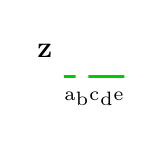
\begin{tikzpicture}
        \begin{axis}[
            ybar,
            axis y line=none,
            axis x line=bottom,
            axis line style={draw=none},
            ymin=0,
            ymax=100,
            width=2.2cm,
            height=2.2cm,
            bar width=1.5mm,
            xtick={a,b,c,d,e},
            xtick style={draw=none},
            symbolic x coords={a,b,c,d,e},
            xticklabel style={font=\scriptsize, anchor=north, yshift=-2pt},
            tick align=inside,
            enlarge x limits=0,
            clip=false,
        ]
            \addplot+[draw=none, fill=none, forget plot] coordinates {(e,100)};
            \addplot+[draw=green!80!black, very thick] coordinates {
            (a,0) (c,0) (d,0) (e,0)
            };

            % Label
            \node[
            anchor=south east,
            font=\scriptsize\bfseries,
            xshift=-1mm, yshift=-5mm
            ] at (current axis.north west) {Z};

        \end{axis}
    \end{tikzpicture}
}

% endregion


\begin{tikzpicture}[node distance=10pt and 20pt, thick]
    
    % Standard CP messaging
    \node (leftPicture) at (0,0) {
        \begin{tikzpicture}[node distance=10pt and 20pt, thick]
            \useasboundingbox (0,0) rectangle (5.5,2);
            % Left side: stacked bar plots with labels
            \matrix (left)[
                matrix of nodes,
                nodes={anchor=west},
                row sep=10pt,
                inner sep=0pt
            ] {
                \node {\blueCPX}; \\
                \node {\blueCPY}; \\ 
                \node {\blueCPZ}; \\
            };
            % Draw blue bounding box around left matrix
            \node[draw=blue, thick, inner sep=5pt, fit=(left)] (blueBox) {};
        
            % Right side: same matrix as left, shifted right of middle
            \matrix (right)[
                matrix of nodes,
                nodes={anchor=west},
                row sep=10pt,
                inner sep=0pt,
                right=4cm of left.center
            ] {
                \node {\redCPX}; \\
                \node {\redCPW}; \\
                \node {\redCPZ}; \\
            };
            % Draw red bounding box around left matrix
            \node[draw=red, thick, inner sep=5pt, fit=(right)] (redBox) {};
            
            \def\arrowSideGap{3mm}
            \def\arrowMidGap{0.75}
            \def\scale{0.75}
            \draw[->, thick]
                ([xshift=\arrowSideGap]blueBox.east |- 0, \arrowMidGap) --
                ([xshift=-\arrowSideGap]redBox.west |- 0, \arrowMidGap) 
                node[pos=0.25, above, yshift=-2mm] 
                {\textbf{X $\neq$ c}};
            \draw[->, thick]
                ([xshift=-\arrowSideGap]redBox.west |- 0, -\arrowMidGap) --
                ([xshift=\arrowSideGap]blueBox.east |- 0, -\arrowMidGap)
                node[pos=0.25, above, yshift=-2mm]
                {\textbf{Z $\neq$ b}};
        \end{tikzpicture}
    };
    
    % CPBP marginal messaging
    \node (rightPicture) [right=0mm of leftPicture.east] {
        \begin{tikzpicture}[node distance=10pt and 20pt, thick]
            \useasboundingbox (0,0) rectangle (5.5,2);
            % Left side: stacked bar plots with labels
            \matrix (left)[
                matrix of nodes,
                nodes={anchor=west},
                row sep=10pt,
                inner sep=0pt
            ] {
                \node {\blueGraphX}; \\
                \node {\blueGraphY}; \\ 
                \node {\blueGraphZ}; \\
            };
            % Draw blue bounding box around left matrix
            \node[draw=blue, thick, inner sep=5pt, fit=(left)] (blueBox) {};
        
            % Right side: same matrix as left, shifted right of middle
            \matrix (right)[
                matrix of nodes,
                nodes={anchor=west},
                row sep=10pt,
                inner sep=0pt,
                right=4cm of left.center
            ] {
                \node {\redGraphX}; \\
                \node {\redGraphW}; \\
                \node {\redGraphZ}; \\
            };
            % Draw red bounding box around left matrix
            \node[draw=red, thick, inner sep=5pt, fit=(right)] (redBox) {};
            
            \def\arrowSideGap{3mm}
            \def\arrowMidGap{0.75}
            \def\scale{0.75}
            \draw[->, thick]
                ([xshift=\arrowSideGap]blueBox.east |- 0, 1 + \arrowMidGap) --
                ([xshift=-\arrowSideGap]redBox.west |- 0, 1 + \arrowMidGap) 
                node[pos=0.25, above, yshift=-2mm] 
                {\scalebox{\scale}{\blueGraphX}};
            \draw[->, thick]
                ([xshift=-\arrowSideGap]redBox.west |- 0, \arrowMidGap) -- 
                ([xshift=\arrowSideGap]blueBox.east |- 0, \arrowMidGap)
                node[pos=0.25, above, yshift=-2mm]
                {\scalebox{\scale}{\redGraphX}};
            \draw[->, thick]
                ([xshift=\arrowSideGap]blueBox.east |- 0,-\arrowMidGap) --
                ([xshift=-\arrowSideGap]redBox.west |- 0,-\arrowMidGap)
                node[pos=0.25, above, yshift=-2mm]
                {\scalebox{\scale}{\blueGraphZ}};
            \draw[->, thick]
                ([xshift=-\arrowSideGap]redBox.west |- 0,-1 - \arrowMidGap) --
                ([xshift=\arrowSideGap]blueBox.east |- 0,-1 - \arrowMidGap)
                node[pos=0.25, above, yshift=-2mm]
                {\scalebox{\scale}{\redGraphZ}};
        \end{tikzpicture}
    };
    

\end{tikzpicture}
